% Session 2 - Rebalancing engine as a horizontal pipeline.
% Build:  pdflatex Fig-RebalancingEngine-Architecture.tex
%         pdf2svg Fig-RebalancingEngine-Architecture.pdf Fig-RebalancingEngine-Architecture.svg
\documentclass[tikz,border=10pt]{standalone}
\usepackage{tikz}
\usepackage{amsmath,amssymb}
\usepackage[T1]{fontenc}
\usepackage{lmodern}
\usepackage{microtype}
\usetikzlibrary{positioning,arrows.meta,shapes.geometric,calc,decorations.markings,backgrounds,fit,shadows.blur}

% --- Per-stage palette: saturated 800-weight border + 100-weight fill ---
\definecolor{obsBorder}{HTML}{1E40AF}    \definecolor{obsFill}{HTML}{DBEAFE}
\definecolor{oriBorder}{HTML}{B31B1B}    \definecolor{oriFill}{HTML}{FEE2E2}
\definecolor{decBorder}{HTML}{5B21B6}    \definecolor{decFill}{HTML}{EDE9FE}
\definecolor{actBorder}{HTML}{15803D}    \definecolor{actFill}{HTML}{DCFCE7}

% --- Neutral typography colors ---
\definecolor{ink}{HTML}{1F2937}
\definecolor{rule}{HTML}{4B5563}
\definecolor{rulesoft}{HTML}{9CA3AF}
\definecolor{paper}{HTML}{FFFFFF}

\newcommand{\stagehead}[2]{{\huge\bfseries\scshape\color{#1} #2}}
\newcommand{\stagesublabel}[1]{{\itshape\large\color{rule} #1}}
\newcommand{\aibadge}[1]{{\itshape\large\color{oriBorder} #1}}
\newcommand{\stagerule}[1]{\par\vspace{4pt}\textcolor{#1}{\rule{\linewidth}{0.7pt}}\par\vspace{8pt}}

\begin{document}
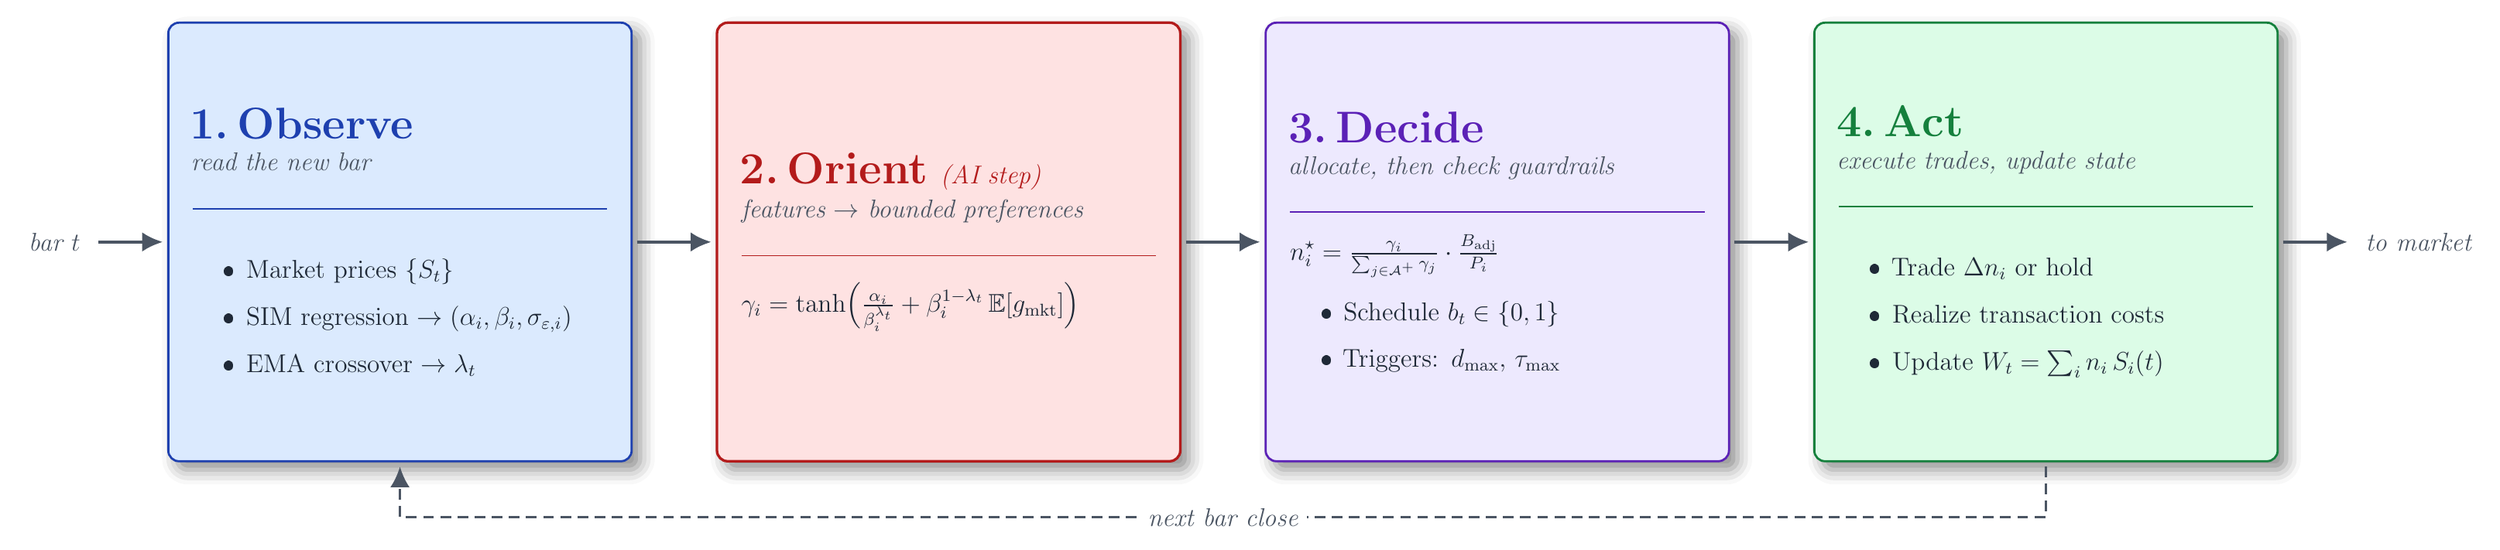
\begin{tikzpicture}[
    >={Latex[length=3.4mm,width=3.2mm]},
    every node/.style={font=\large, text=ink},
    stage/.style={
        rectangle, rounded corners=5pt, line width=1.0pt,
        minimum width=76mm, minimum height=72mm,
        align=left, text width=68mm, inner sep=10pt,
        blur shadow={shadow xshift=1.4mm, shadow yshift=-1.4mm,
                     shadow opacity=45, shadow blur radius=2.4mm},
    },
    obsbox/.style={stage, draw=obsBorder, fill=obsFill},
    oribox/.style={stage, draw=oriBorder, fill=oriFill, line width=1.2pt},
    decbox/.style={stage, draw=decBorder, fill=decFill},
    actbox/.style={stage, draw=actBorder, fill=actFill},
    arr/.style={->, line width=1.6pt, draw=rule, shorten >=2pt, shorten <=2pt},
    feedback/.style={->, line width=1.2pt, draw=rule, dash pattern=on 5pt off 3pt,
                     shorten >=2pt, shorten <=2pt},
]

\def\dx{90mm}

% --- Stage 1: OBSERVE ---
\node[obsbox] (observe) at (0,0) {%
    \stagehead{obsBorder}{1.\ Observe}\\[1pt]
    \stagesublabel{read the new bar}
    \stagerule{obsBorder}
    \begin{itemize}\setlength\itemsep{4pt}\setlength\leftmargini{1.2em}
        \item Market prices $\{S_t\}$
        \item SIM regression $\to (\alpha_i, \beta_i, \sigma_{\varepsilon,i})$
        \item EMA crossover $\to \lambda_t$
    \end{itemize}
};

% --- Stage 2: ORIENT (AI step) ---
\node[oribox] (orient) at (\dx,0) {%
    \stagehead{oriBorder}{2.\ Orient}\enspace\aibadge{(AI step)}\\[2pt]
    \stagesublabel{features $\to$ bounded preferences}
    \stagerule{oriBorder}\vspace{4pt}
    $\displaystyle \gamma_i = \tanh\!\Big(\tfrac{\alpha_i}{\beta_i^{\lambda_t}} + \beta_i^{1-\lambda_t}\,\mathbb{E}[g_{\mathrm{mkt}}]\Big)$
};

% --- Stage 3: DECIDE ---
\node[decbox] (decide) at (2*\dx,0) {%
    \stagehead{decBorder}{3.\ Decide}\\[1pt]
    \stagesublabel{allocate, then check guardrails}
    \stagerule{decBorder}
    $\displaystyle n_i^{\star} = \tfrac{\gamma_i}{\sum_{j\in\mathcal{A}^+}\gamma_j} \cdot \tfrac{B_{\mathrm{adj}}}{P_i}$\\[6pt]
    \begin{itemize}\setlength\itemsep{4pt}\setlength\leftmargini{1.2em}
        \item Schedule $b_t \in \{0, 1\}$
        \item Triggers: $d_{\max}$, $\tau_{\max}$
    \end{itemize}
};

% --- Stage 4: ACT ---
\node[actbox] (act) at (3*\dx,0) {%
    \stagehead{actBorder}{4.\ Act}\\[1pt]
    \stagesublabel{execute trades, update state}
    \stagerule{actBorder}
    \begin{itemize}\setlength\itemsep{4pt}\setlength\leftmargini{1.2em}
        \item Trade $\Delta n_i$ or hold
        \item Realize transaction costs
        \item Update $W_t = \sum_i n_i\, S_i(t)$
    \end{itemize}
};

% --- Forward arrows between stages ---
\draw[arr] (observe.east)  -- (orient.west);
\draw[arr] (orient.east)   -- (decide.west);
\draw[arr] (decide.east)   -- (act.west);

% --- Feedback loop: Act -> Observe (next bar) ---
\draw[feedback]
    (act.south) -- ++(0,-9mm) -| (observe.south);

% --- Feedback label sits on the horizontal stretch of the loop ---
\node[font=\itshape\large, text=rule, fill=paper, inner xsep=4pt, inner ysep=1pt]
  at ($(observe.south)!0.5!(act.south) + (0,-9mm)$)
  {next bar close};

% --- Bar-of-data inflow indicator on the left ---
\draw[arr] ($(observe.west) + (-12mm,0)$) -- (observe.west);
\node[font=\itshape\large, text=rule, anchor=east]
  at ($(observe.west) + (-13mm,0)$) {bar $t$};

% --- Trade outflow indicator on the right ---
\draw[arr] (act.east) -- ++(12mm,0);
\node[font=\itshape\large, text=rule, anchor=west]
  at ($(act.east) + (13mm,0)$) {to market};

\end{tikzpicture}
\end{document}
